\section{Taxonomy of Contributions}\label{sec:taxonomy-of-contributions}
\begin{figure}[!ht]
    \centering
    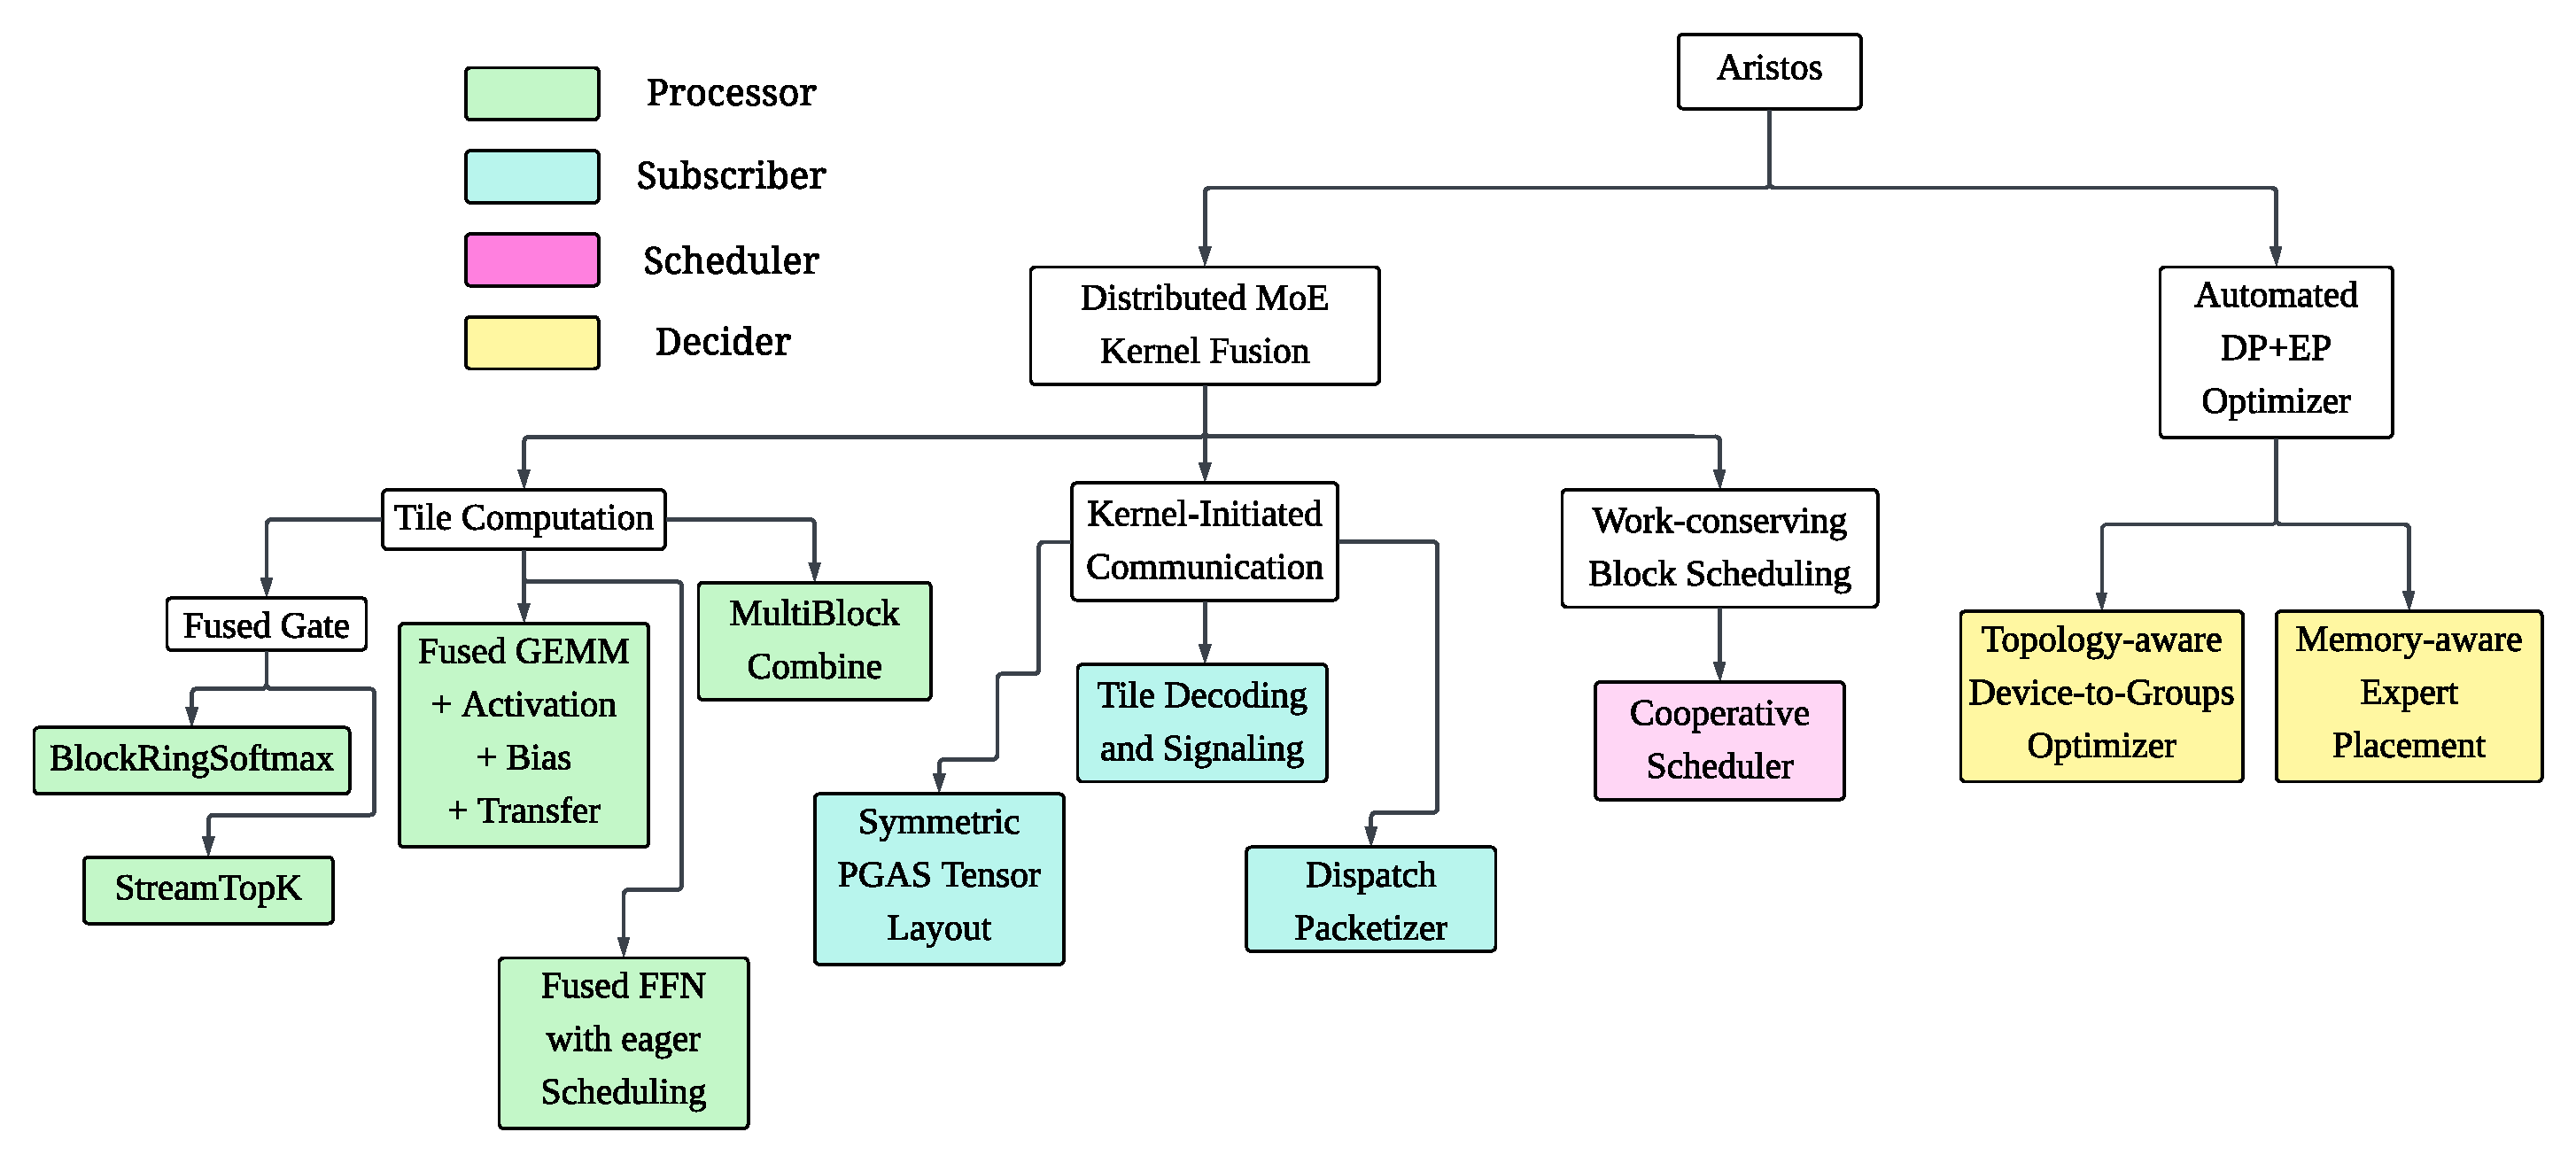
\includegraphics[width=5.5in,keepaspectratio]{figures/Taxonomy}
    \caption{\emph{Taxonomy of this work's system contributions}.
    Each colored box is a submodule, whose algorithm(s) we explicate in~\S\ref{sec:method}.
        (1) \textcolor{LimeGreen}{Green} boxes encapsulate \emph{tile computational} operations.
        We implement \textbf{fusion} for these operators as post-processing on post-compute \emph{register storage},
        eliding the round-trip to and from GPU HBM memory. (2) \textcolor{Aquamarine}{Blue} boxes indentify
        our asynchronous task/tile dependency management; and \emph{packet-switching} mechanism and
        PGAS tensor layout we leverage to achieve
        \emph{complete communication efficiency}, wherein we transmit no zero-padded bytes over the network.
        (3) The \textcolor{Lavender}{Pink} box identifies a \emph{cooperative, work-conserving scheduler},
        we implement for fast dispatching of tiles to GPU thread blocks. Note that cooperative means
        multithreaded execution.
        (4) \textcolor{yellow}{Yellow} boxes entail optimization algorithms
        we introduce for automated generation of model parallelism strategies that are
        aware of device throughput and network topology, while subject to device memory constraints.
        \textcolor{LimeGreen}{Green}, \textcolor{Aquamarine}{Blue} and \textcolor{Lavender}{Pink} boxes are
        all \emph{in-kernel} submodules comprising a \emph{single, persistent} GPU kernel.
        \textcolor{yellow}{Yellow} boxes are one-shot CPU subroutines.
    }
    \label{fig:taxonomy}
\end{figure}